Spatial Cloaking ist eine Verschleierungstaktik, bei der der Anwender seinen genauen Standort mithilfe von k-anonymity verheimlicht. Das bedeutet, dass versucht wird, eine definierte Fläche zu erzeugen. Diese Fläche soll die Eigenschaft besitzen, dass mindestens k-1 andere Personen sich in dieser aufhalten können. Um dem Anwender eine einfache Möglichkeit zu bieten, seinen Standort zu verschleiern, wird ein sogenannter location anonymizer zwischen den Nutzer und den LBS geschaltet. Ein location anonymizer hat die Aufgabe, den Standort des Nutzers zu verheimlichen.

Stellt der Nutzer nun eine Anfrage an einen Service, wie z. B. \glqq Zeige mir alle Restaurants in der Nähe\grqq, dann schickt das Endgerät seinen genauen Standort mit Anfrage an den location anonymizer. Dieser erzeugt nun ein Gebiet, in welchem der Nutzer sich befindet und welches gleichzeitig die Sicherheitskriterien erfüllt. Bei den Sicherheitskriterien handelt es sich primär um die Größe des zu erzeugenden Gebietes und wie viele weitere Personen sich in diesem aufhalten sollen. Anschließend stellt der location anonymizer die Anfrage an den vom Nutzer spezifizierten Service, jedoch wird lediglich das erzeugte Gebiet und nicht die genaue Position des Anwenders übermittelt. Als Antwort erhält der location anonymizer nun alle Restaurants in dem Gebiet und kann dem Nutzer alle daraus relevanten Informationen zur Verfügung stellen.

Wird im Folgenden von einem Gebiet oder Areal gesprochen, welches von einem location anonymizer erzeugt wurde, so spricht man von einer Cloaked-Area. Um eine Cloaked-Area zu erzeugen, gibt es verschiedene Methoden. Zum einen kann der Anonymizer, wenn er eine Cloaked-Area erzeugen möchte, bei jeder Anfrage an das LBS dieselben Partner verwenden, zum anderen hat er die Möglichkeit, sich jedes Mal neue Partner für die Erzeugung einer Cloaked-Area zu suchen. Jedoch ist es bei beiden Methoden nicht ausreichend, zu einem bestimmten Abfragezeitpunkt an den angefragten Service k-anonymity zu gewährleisten \cite{Chow2011}. Im Folgenden werden zwei verschiedene Angriffe auf das Spatial Cloaking Verfahren erläutert und wie der Nutzer sich gegen diese verteidigen kann. 
\subsubsection{Trajectory tracing Attacke} 
In \cite{Chow2011} wird ein Angriff auf Spatial Cloaking vorgestellt. Diese wird angewendet, wenn der Nutzer von Spatial Cloaking beim Erzeugen einer Cloaked-Area immer die selben Partner benutzt. Der dort vorgestellte Angriff wird trajectory tracing Attacke genannt. Dabei versucht der Angreifer, den Anwender anhand seiner Anfragen an das LBS zu identifizieren, indem ein Schnittpunkt zwischen dem aktuellen Gebiet und dem Gebiet, in welchem er sich seit der letzten Anfrage befinden muss, errechnet wird. 
\begin{figure}[!h]
		\centering
		\subfloat{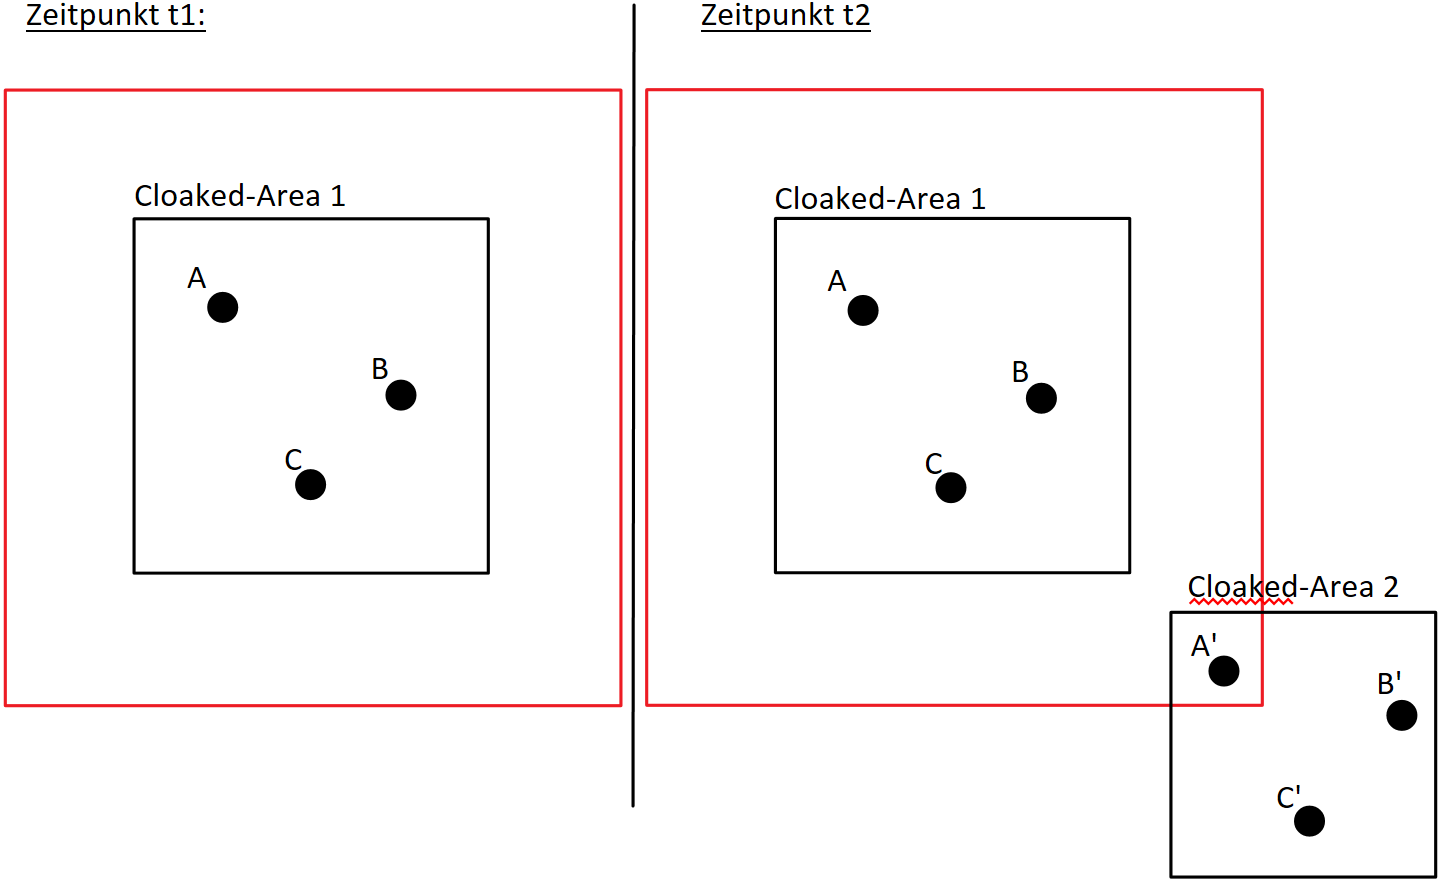
\includegraphics[width=7cm]{Bilder/Alex/TrajectoryTracingAttacke.png}\label{figA}}
		\caption{Trajectory tracing Attacke}
		\label{fig_chow2011_traj-tracing-att}
\end{figure}
Angenommen es wird zum Zeitpunkt t$_{1}$ eine Cloaked-Area 1 mit den Nutzern A, B und C erstellt und die Bewegungsgeschwindigkeit des Opfers (im Beispiel 'Nutzer A') ist dem Angreifer bekannt. So kann der Angreifer zu jedem beliebigen nachfolgendem Zeitpunkt t$_{n}$ das maximale Gebiet errechnen, in welchem sich der Nutzer aufhalten kann. Dies geschieht unter der Berücksichtigung von Straßen- und Geländeverhältnissen. In Abbildung \ref{fig_chow2011_traj-tracing-att} wird diese maximale Grenze durch das rote Quadrat verdeutlicht. Daraus ergibt sich zum Zeitpunkt t$_{n}$ eine maximale Grenze. Zu einem Zeitpunkt t$_{2}$ formt die Gruppe, bestehend aus A, B und C, eine neue Spatial-Cloaking-Area 2 und stellt erneut eine Anfrage an das LBS. Der Angreifer hat nun die Möglichkeit die maximale Grenze vom Zeitpunkt t$_{1}$ mit der Spatial-Cloaking-Area 2 zu schneiden. Sollte nur ein Nutzer in dieser Schnittmenge enthalten sein, so hat der Angreifer Nutzer A erfolgreich identifiziert.

Der position anonymizer hat zwei Möglichkeiten sich gegen diese Art von Angriff zu wehren. Bei beiden Gegenmaßnahmen muss der Nutzer die maximale Grenze in Abhängigkeit des Zeitpunkt t$_{1}$ berechnen. Anschließend kann er entweder die in \cite{Chow2011} vorgestellte \textbf{patching technique} oder die \textbf{delaying technique} anwenden. 
\begin{itemize} 
\item{Delaying technique} funktioniert, indem der Anwender eine Anfrage zu einem beliebigen Zeitpunkt t$_{2}$ an das LBS formuliert. Würde der Anonymizer nun direkt die Anfrage abschicken, dann könnte der Angreifer die trajectory tracing Attacke durchführen und so den Nutzer identifizieren. Um dies zu verhindern muss die Anfrage verzögert werden. 
\begin{figure}[!h]
		\centering
		\subfloat{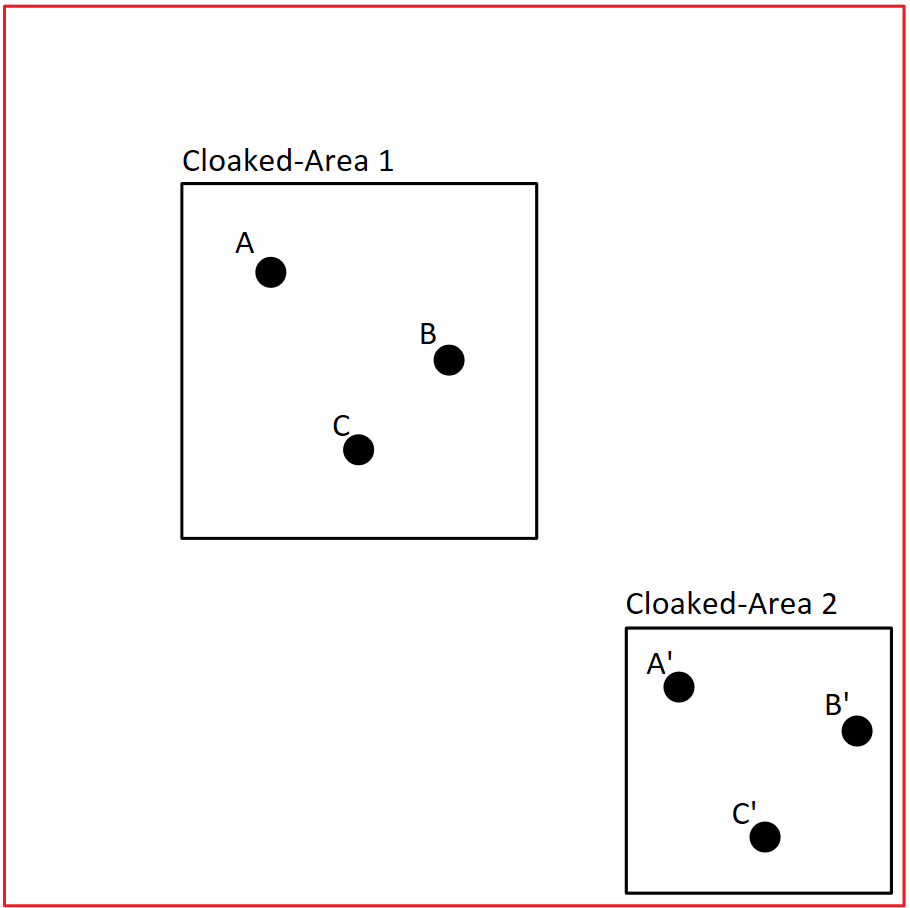
\includegraphics[width=4.5cm]{Bilder/Alex/DelayingTechnique.png}\label{figA}}
		\caption{Delaying technique}
		\label{fig_chow2011_delaying-tech}
\end{figure}
Die Verzögerung muss so groß gewählt werden, bis die maximale Grenze von t$_{1}$ so stark angewachsen ist, dass die gebildete Cloaked-Area 2 zum Zeitpunkt t$_{2}$ komplett von der maximalen Grenze überlappt wird. Wird nun die Schnittmenge aus der Cloaked-Area 2 und der maximalen Grenze zum Zeitpunkt t$_{1}$ errechnet, so stellt diese das Ergebnis der maximalen Grenze zu t$_{1}$ dar. Problematisch sind bei diesem Lösungsansatz jedoch, dass Anfragen an das LBS nicht zeitnah beantwortet werden können. Es muss eben gewartet werden, bis die maximale Grenze die Cloaked-Area 2 überlappt. 
\item{Patching technique} kombiniert die maximale Grenze basierend auf dem Zeitpunkt t$_{1}$ mit der Cloaked-Area 2, um eine neue Cloaked-Area zu erhalten. Zu sehen ist dies in Abbildung \ref{fig_chow2011_patching-tech}.
\begin{figure}[!h]
		\centering
		\subfloat{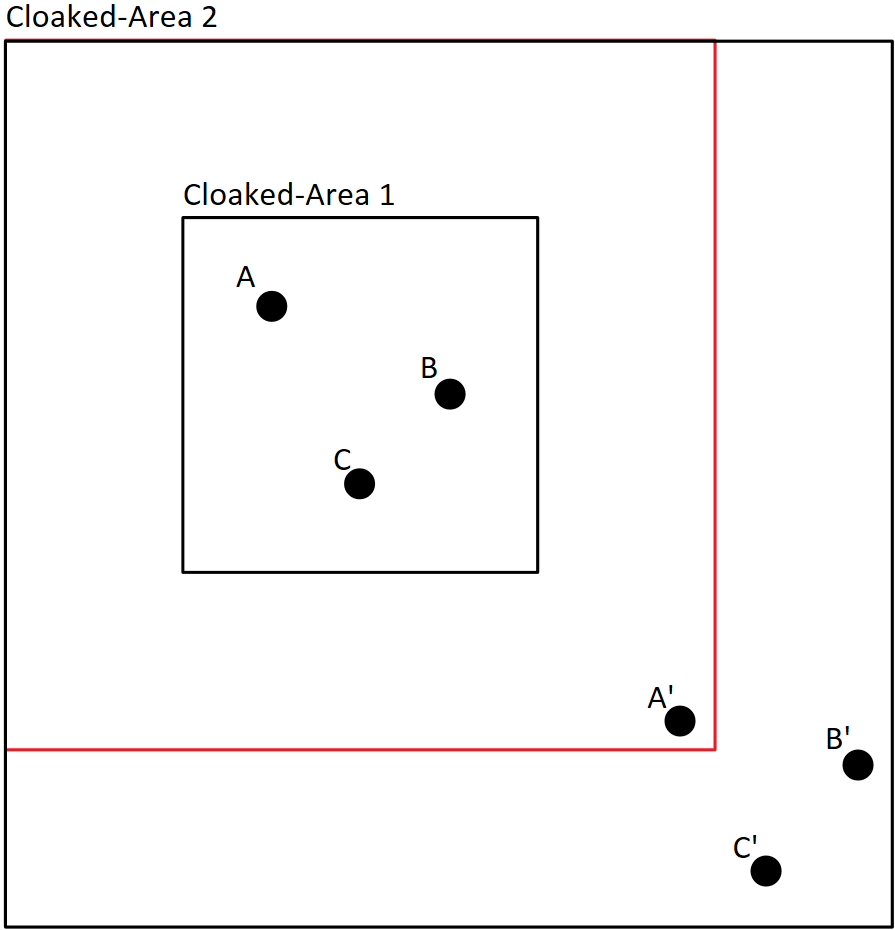
\includegraphics[width=4.5cm]{Bilder/Alex/PatchingTechnique.png}\label{figA}}
		\caption{Patching technique}
		\label{fig_chow2011_patching-tech}
\end{figure}
Diese Cloaked-Area kann anschließend als Grundlage der Anfrage an das LBS benutzt werden. Bei dieser Methode leidet jedoch die Genauigkeit der Ergebnisse, da diese neue Cloaked-Area sehr groß werden kann, wenn sich die Personen der Cloaked-Area voneinander weg bewegen.  
\end{itemize} 
\subsubsection{Anonymity-set tracing Attacke} 
In \cite{chow2007} wird eine weitere Möglichkeit erläutert, Spatial Cloaking anzugreifen. Diese Art der Attacke wird auch anonymity-set tracing Attacke genannt. Damit sie erfolgreich durchgeführt werden kann, muss das Opfer bei jeder Anfrage an das LBS die Cloaked-Area mit anderen Partnern neu erzeugen. Hat der Angreifer nun zwei Anfragen an das LBS mitgelesen, so kann er vergleichen, welche Personen in der Cloaked-Area gleich geblieben und welche neu hinzugekommen sind, bzw. den Bereich verlassen haben. Tritt der Fall ein, dass nur noch eine einzelne Person über alle Cloaked-Areas konstant bleibt, so ist diese Person das Opfer des Sicherheitsangriffs.

Im Folgenden werden nun drei verschiedene Ansätze des Spatial Cloaking aus \cite{Chow2011} näher betrachtet. Um den eben genannten Angriffen entgegen wirken zu können, müssen diese mit den eben erläuterten Techniken verknüpft werden. Darauf wird in der folgenden Ausführung jedoch verzichtet. Bei allen Ansätzen ist es notwendig, dass ein ein location anonymizer zwischen dem LBS und dem Anwender implementiert ist. Dieser stellt die eigentliche Anfrage an das LBS, um eine Anonymität des Nutzern zu gewährleisten und um die Cloaked-Area zu erzeugen. 
\subsubsection{Group-based Ansatz} 
Der group-based Ansatz ist eine Verschleierungstaktik, welche auf Real-Time Daten aufbaut. Stellt dieselbe Person zwei Abfragen an den location anonymizer, so wird die Cloaked-Area immer mit denselben Personen erzeugt, welche auch schon bei der ersten Cloaked-Area involviert waren. So wird sichergestellt, dass die anonymity-set tracing Attacke für einen potentiellen Angreifer nicht anwendbar ist. Sucht Person A z. B. alle Restaurants in seiner Nähe, so formt der position anonymizer eine Cloaked-Area mit den Personen B und C. Damit Person A nun weitere Anfragen, wie z. B. \glqq Zeige mir alle Kaffees in der Nähe\grqq~ stellen kann, müssen Personen B und C ebenfalls ihre Position dem position anonymizer jederzeit zur Verfügung stellen. 

Wenn diese Art von Ansatz gewählt wird, um die eigene Position zu verschlüsseln, so muss man jedoch Nachteile berücksichtigen. Der location anonymizer muss die Position von allen Nutzern zu jedem Zeitpunkt kennen. Das kann vor allem bei mobilen Endgeräten Probleme mit der Akkulaufzeit verursachen.  
\subsubsection{Distortion-based Ansatz} 
Der distortion-based Ansatz ist eine Erweiterung des group-based Ansatzes. Er versucht das Problem, dass die Nutzer gezwungen sind, ihre Position immer aktuell zu halten, aus dem group-based Ansatz zu beheben. 
\begin{figure}[!h]
		\centering
		\subfloat{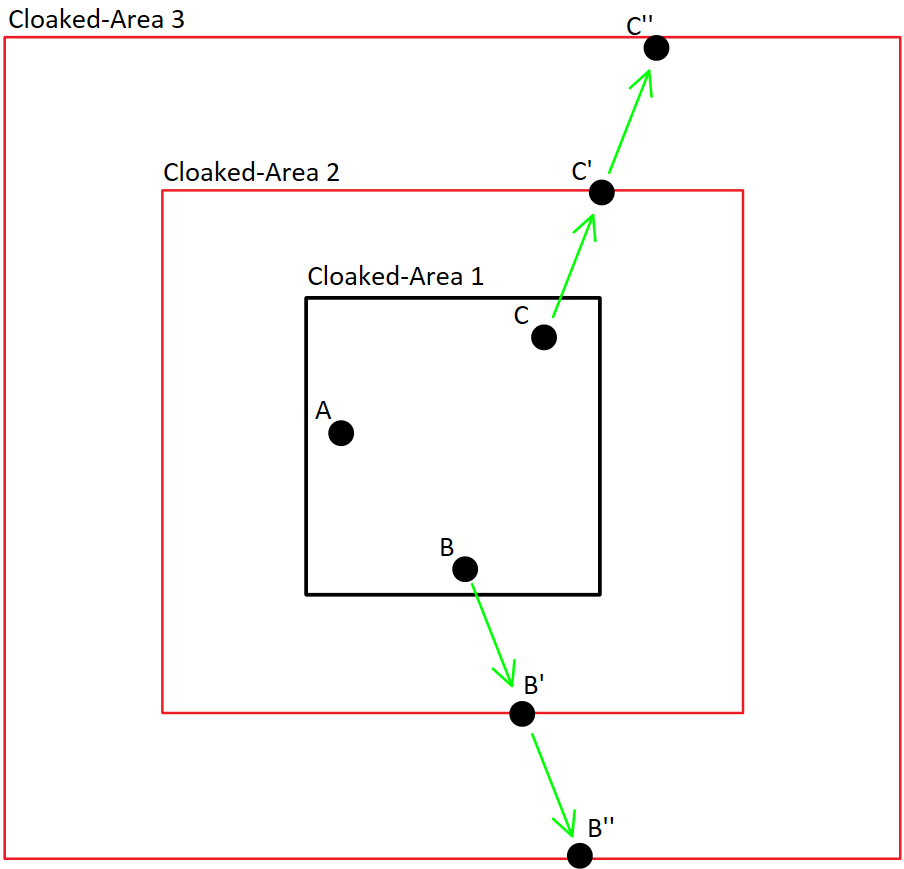
\includegraphics[width=4.5cm]{Bilder/Alex/DistortionBased.png}\label{figA}}
		\caption{Distortion-based Ansatz}
		\label{fig_chow2011_Distortion-Ansatz}
\end{figure}
In Abbildung \ref{fig_chow2011_Distortion-Ansatz} ist zu erkennen, wie Person A eine Anfrage an ein LBS stellt und der location anonymizer dazu eine Cloaked-Area erzeugt. Zu diesem Zeitpunkt merkt sich der location anonymizer die Geschwindigkeit jeder Person die zu dieser Gruppe gehört. Anhand der Geschwindigkeiten kann der location anonymizer nun schätzen wo sich Person B und C befinden könnten. Mithilfe dieser Schätzungen und der Position von A können nun Cloaked-Areas erzeugt werden, ohne dass Person B und C dazu gezwungen werden ihre Position zu jeder Zeit bereit zu stellen.
\subsubsection{Predication-based Ansatz} 
Dieser Ansatz benötigt keine Echtzeitinformationen von anderen Nutzern. Er ist besonders in Gebieten hilfreich, bei denen sich in der Umgebung des Anfragestellers nicht genug weitere Personen befinden, um k-anonymity zu gewährleisten. Ein für ein bestimmtes Gebiet zuständiger location anonymizer speichert sich dazu die Trajectories von verschiedenen Nutzern, welche sich zu einer beliebigen Zeit eingeloggt haben. Soll der location anonymizer nun für einen Nutzer k-anonymity gewährleisten und eine Cloaked-Area erstellen, hat aber nicht genug Personen in dem entsprechendem Gebiet, so greift dieser auf zuvor gespeicherte Trajectories zurück. Dabei versucht der location anonymizer anhand der Geschwindigkeit des Nutzers vorherzusagen, welche Footprints vergangener Aufzeichnungen sich am besten eignen um eine Cloaked-Area zu erstellen. Dies ist in Abbildung \ref{fig_chow2011_PredicationBased-Ansatz} verdeutlicht. Person A ist dabei der Nutzer des LBS und vorangegangene Trajectories wurden durch Person B und C (blaue und pinke Punkte) erzeugt. Problematisch ist jedoch die optimale Fläche der Cloaked-Area zu berechnen, da ein Suchalgorithmus implementiert werden muss, welcher die besten Positionen von aufgezeichneten Trajectories ermittelt. Hier sollte mit einer guten Heuristik gearbeitet werden. 
\begin{figure}[!h]
		\centering
		\subfloat{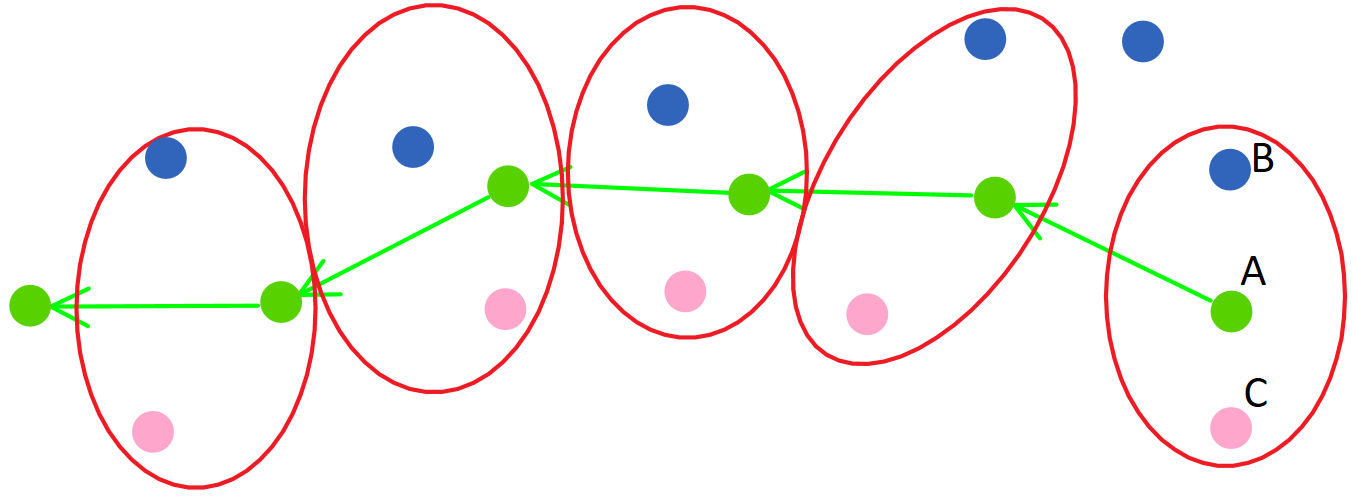
\includegraphics[width=6.0cm]{Bilder/Alex/PredicationBased.png}\label{figA}}
		\caption{Predication-based Ansatz}
		\label{fig_chow2011_PredicationBased-Ansatz}
\end{figure}